\documentclass[11pt,spanish,a4paper]{article}

% Versión 1.er cuat 2021 Víctor Bettachini < vbettachini@unlam.edu.ar >

\usepackage[T1]{fontenc}
\usepackage[utf8]{inputenc}

\usepackage[spanish, es-tabla]{babel}
% \def\spanishoptions{argentina} % Was macht dass?
% \usepackage{babelbib}
% \selectbiblanguage{spanish}
% \addto\shorthandsspanish{\spanishdeactivate{~<>}}


\usepackage{graphicx}
\graphicspath{{./figuras/}{../LaTeX/}{../figurasLaTeX/}}
% \usepackage{float}

\usepackage[arrowdel]{physics}
\newcommand{\pvec}[1]{\vec{#1}\mkern2mu\vphantom{#1}}
% \usepackage{units}
\usepackage[separate-uncertainty= true, multi-part-units= single, range-units= single, range-phrase= {~a~}, locale= FR]{siunitx}
\usepackage{isotope} % $\isotope[A][Z]{X}\to\isotope[A-4][Z-2]{Y}+\isotope[4][2]{\alpha}

\usepackage{tasks}
\usepackage[inline]{enumitem}
% \usepackage{enumerate}

\usepackage{hyperref}

% \usepackage{amsmath}
% \usepackage{amstext}
% \usepackage{amssymb}

\usepackage{tikz}
\usepackage{tikz-3dplot}
\usepackage{tikz-dimline}
\usetikzlibrary{calc}
% \usetikzlibrary{math}
\usetikzlibrary{arrows.meta}
\usetikzlibrary{snakes}
\usetikzlibrary{decorations}
\usetikzlibrary{decorations.pathmorphing}
\usetikzlibrary{patterns}

\usepackage[hmargin=1cm,vmargin=3cm, top= 0.75cm,nohead]{geometry}

\usepackage{lastpage}
\usepackage{fancyhdr}
\pagestyle{fancyplain}
\fancyhf{}
\setlength\headheight{28.7pt} 
\fancyhead[LE, LO]{\textbf{Mecánica Analítica Computacional} }
% \fancyhead[LE, LO]{\textbf{Mecánica General} }
\fancyhead[RE, RO]{\href{https://ingenieria.unlam.edu.ar/}{$\vcenter{\hbox{
\includegraphics[height=1cm]{ambos.pdf}}}$}}
\fancyfoot{\href{https://creativecommons.org/licenses/by-nc-sa/4.0/deed.es_ES}{$\vcenter{\hbox{
\includegraphics[height=0.4cm]{by-nc-sa_80x15.pdf}}}$} \href{https://ingenieria.unlam.edu.ar/}{DIIT - UNLaM}}
\fancyfoot[C]{ {\tiny Actualizado al \today} }
\fancyfoot[RO, LE]{Pág. \thepage/\pageref{LastPage}}
\renewcommand{\headrulewidth}{0pt}
\renewcommand{\footrulewidth}{0pt}


\begin{document}
\begin{center}
  \textsc{\large Mecánica general}\\
  \textsc{\large Cuerpo rígido | Tensores de inercia}
\end{center}

% De poder resolver estos problemas en forma autónoma puede asumir que adquirió los conocimientos mínimos sobre los temas abordados en la semana. No dude en consultar a docentes y compañeros si no puede terminarlos.
Los problemas marcados con (*) son opcionales.

\begin{enumerate}

% \vspace{-.5cm}
% \section*{Tensores de inercia}


\item Se tiene una barra de \(m= \SI{1}{\kilo\gram}\) de sección despreciable frente a \(l= \SI{1}{\metre}\).
De alinear un eje (\(\hat{z}\)) con ella, 
\begin{tasks}(2)
	\task	¿cuales son sus momentos de inercia?,
	\task ¿existen los productos de inercia? 
\end{tasks}


\item
Dibuje sistemas de ejes conveniente para calcular momentos de inercia.
\vspace{-1.1cm}
\begin{tasks}(4)
	\task 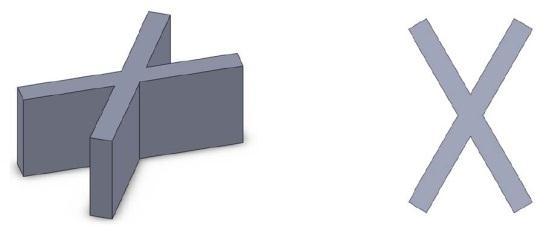
\includegraphics[width=0.15\textwidth]{o-000}
	\task 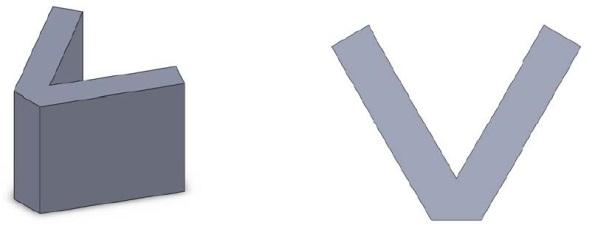
\includegraphics[width=0.15\textwidth]{o-001}
	\task 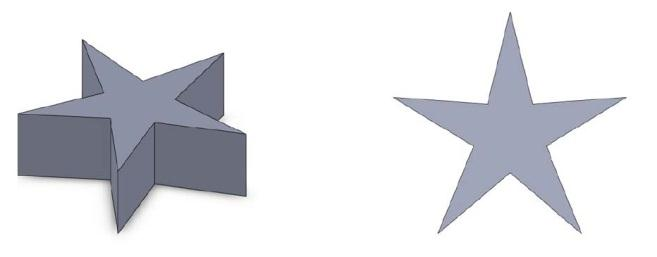
\includegraphics[width=0.15\textwidth]{o-002}
	\task 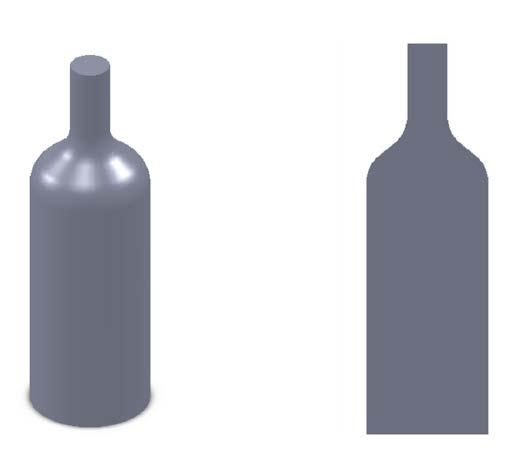
\includegraphics[width=0.15\textwidth]{o-003}
\end{tasks}



\item 
\begin{minipage}[t][4.5cm]{0.7\textwidth}
Calcule para el sistema de ambas $m$ (la masa de brazos y ejes es despreciable)
\begin{tasks} 
	\task momento de inercia \(\overline{\overline{I}}\) respecto a A,
	\task momento angular $\vec{L}\bigg\rvert_A = \overline{\overline{I}} \vec{\Omega}$ y torque $\vec{\tau} = \dot{\vec{L}}$.
\end{tasks}
La porción vertical de la barra se mantiene con rulemanes que impiden su movimiento vertical, pero posibilitan que el eje rote sin fricción con velocidad angular $\Omega$ respecto el marco inercial $O_{xyz}$.
\end{minipage}
\begin{minipage}[c][1cm][t]{0.25\textwidth}
	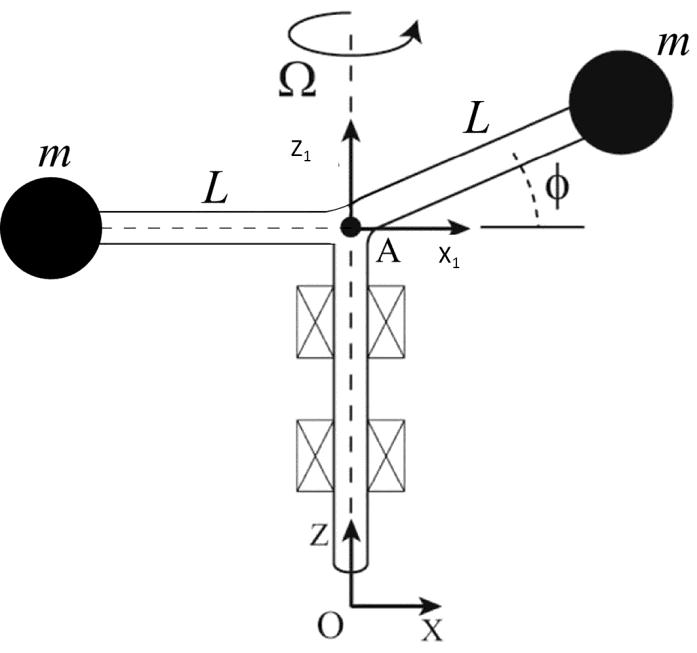
\includegraphics[width=\textwidth]{o-021}
\end{minipage}



\item Calcule los momentos de inercia para una molécula de \isotope{H_2O}.\\
En CNPT se abre con un ángulo de \ang{104,5;;} y median \SI{95.84}{\pico\metre} entre \isotope{O} y \isotope{H}.



\item 
\begin{minipage}[t][3.7cm]{0.6\textwidth}
% \begin{minipage}[t][3.5cm]{0.7\textwidth}
Tensor de inercia de un cubo con arista \(b\).
% \textbf{Marion e.g. 11-35 y 11-6} Tensor de inercia de un cubo con arista \(b\).
	
Encuentre: 
\begin{enumerate}
	\item Calcule el tensor de inercia desde el sistema con origen en el vértice \(Q\) en el sistema \(X_i\).
	\item Use la forma general del teorema de ejes paralelos de Steiner para calcularlo ahora desde el centro de masa \(O\) para el sistema \(x_i\).
	\end{enumerate}
\end{minipage}
\begin{minipage}[c][1.2cm][t]{0.35\textwidth}
	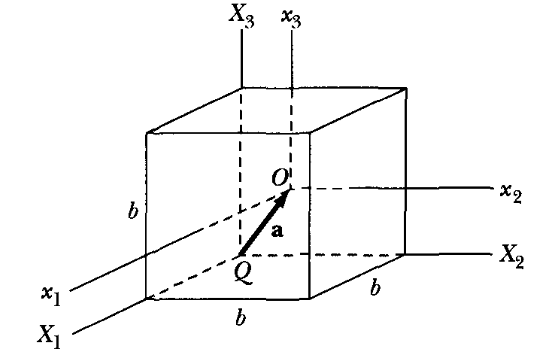
\includegraphics[width=\textwidth]{mFig11-8}
\end{minipage}



\item 
\begin{minipage}[t][3cm]{0.5\textwidth}
En una plancha metálica se calaron dos aberturas en forma simétrica.
Esta \emph{penduléa} desde el punto A.
Calcule el momento de inercia \(I_{zz}\) desde su centro de masa y luego desde A.
\end{minipage}
\begin{minipage}[c][4cm][t]{0.45\textwidth}
	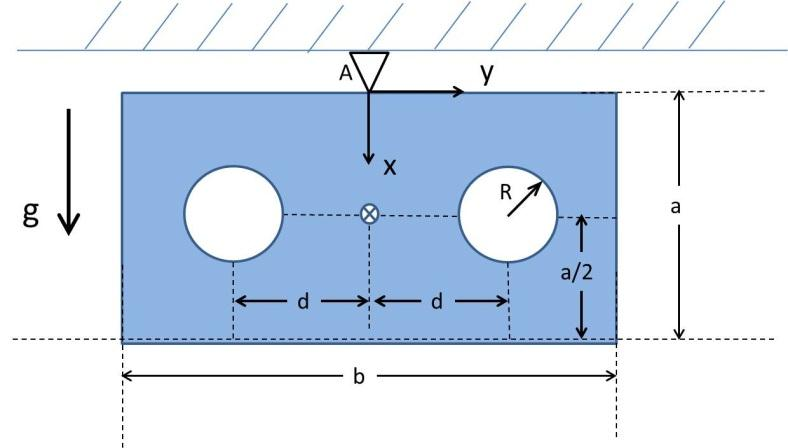
\includegraphics[width=\textwidth]{o-023}
\end{minipage}



\item 
\begin{minipage}[t][1.5cm]{0.65\textwidth}
	Hallar la energía cinética de un cilindro homogéneo de radio \(a\) que rueda en el interior de una superficie cilíndrica de radio \(R\).
	% \textbf{Landau \S 32 6} Hallar la energía cinética de un cilindro homogéneo de radio \(a\) que rueda en el interior de una superficie cilíndrica de radio \(R\).
\end{minipage}
\begin{minipage}[c][1.5cm][t]{0.3\textwidth}
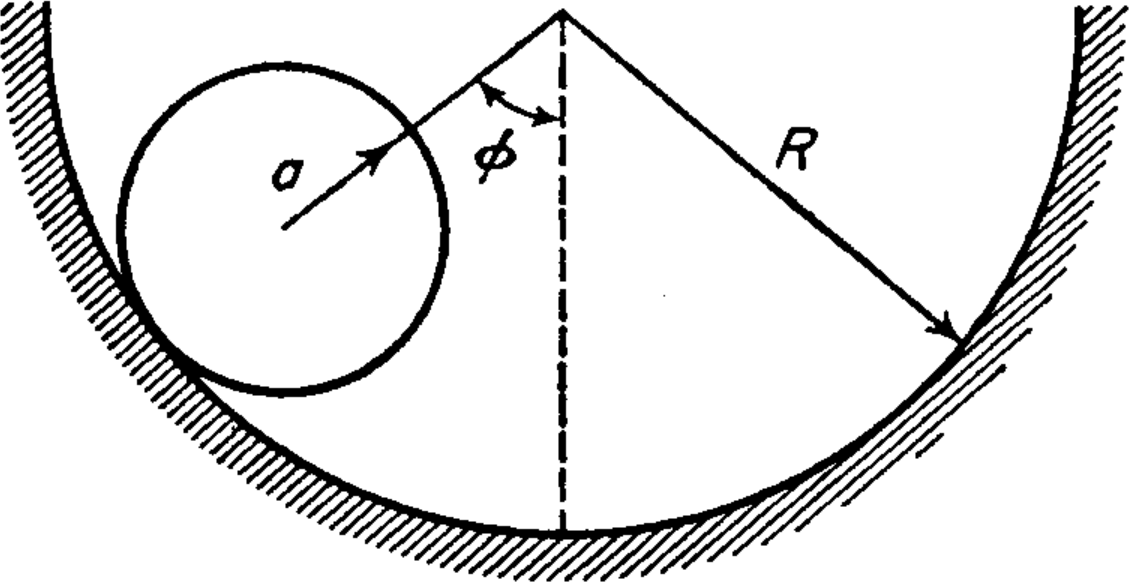
\includegraphics[width=\textwidth]{lFig41}
\end{minipage}



\item 
\begin{minipage}[t][3.5cm]{0.5\textwidth}
(*) Calcule:
	\begin{enumerate}
		% \item \textbf{Landau \S 32 2e} Calcule los momentos principales de inercia de un cono homogéneo de altura \(h\) y radio \(R\).
		\item Momentos principales de inercia de un cono homogéneo de altura \(h\) y radio en su base \(R\).
		\item Energía cinética de dicho cono rodando sobre un plano.
		% \textbf{Landau \S 32 7} Hallar la energía cinética de un cono homogéneo que rueda sobre un plano.
	\end{enumerate}
\end{minipage}
\begin{minipage}[c][1cm][t]{0.45\textwidth}
	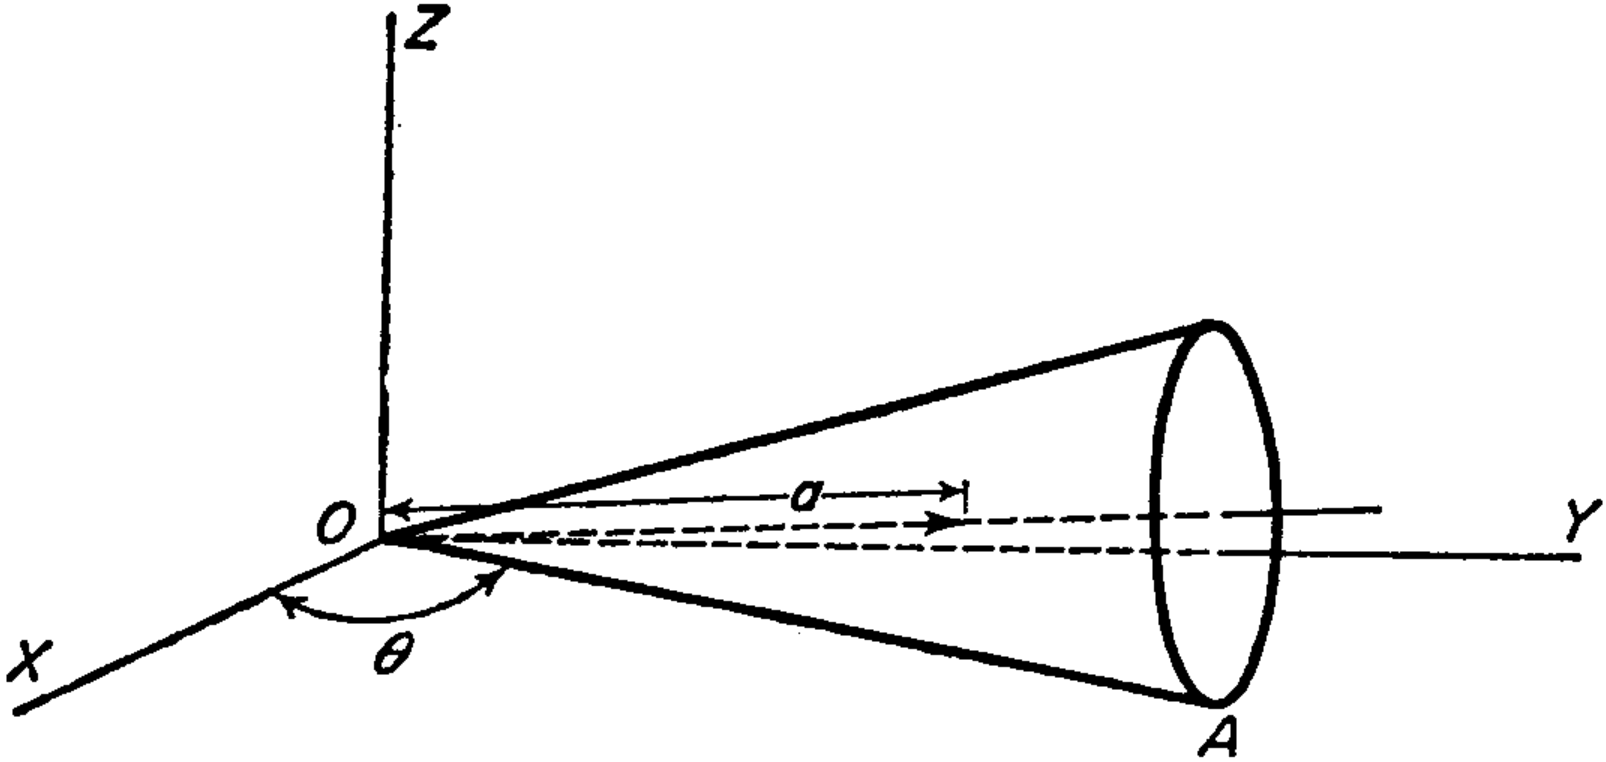
\includegraphics[width=\textwidth]{lFig42}
\end{minipage}




\end{enumerate}
\end{document}
